\chapter{GIT HISTORY}
All source code for the Route Optimizer project is maintained in a centralized Git repository. This ensures rigorous version control, enabling collaborative development and the maintenance of a robust project history. This chapter documents the repository structure, branching strategy, and key development milestones.

\section{Repository Structure}
The repository is organized with a clear separation of concerns, dividing the codebase into frontend and backend directories. This structure allows for independent development, testing, and deployment of the two tiers of the application.

\begin{table}[H]
    \centering
    \renewcommand{\arraystretch}{1.3}
    \small
    \begin{tabular}{|p{4cm}|p{9cm}|}
        \hline
        \textbf{Directory / File} & \textbf{Description} \\
        \hline
        \texttt{Frontend/} & React application source code (Vite-based) \\
        \hline
        \texttt{Frontend/src/components/} & Reusable UI components (common, dashboard, layout) \\
        \hline
        \texttt{Frontend/src/pages/} & Page-level components (Home, Login, Register) \\
        \hline
        \texttt{Frontend/src/utils/} & Utility modules (geocoding, optimizer, weather, places) \\
        \hline
        \texttt{Frontend/src/context/} & React Context providers (AuthContext) \\
        \hline
        \texttt{Backend/} & Express.js API server source code \\
        \hline
        \texttt{Backend/models/} & Mongoose schema definitions (User, Route) \\
        \hline
        \texttt{Backend/routes/} & API route handlers (auth, routes) \\
        \hline
        \texttt{Backend/middleware/} & Authentication middleware (JWT verification) \\
        \hline
        \texttt{Backend/config/} & Database connection configuration \\
        \hline
        \texttt{Backend/server.js} & Express application entry point \\
        \hline
        \texttt{package.json} & Root-level project metadata and scripts \\
        \hline
    \end{tabular}
    \caption{Repository Directory Structure}
    \label{tab:repo_structure}
\end{table}

\section{Version Control Practices}
The following version control practices were followed throughout the development of Route Optimizer:
\begin{itemize}
    \item \textbf{Descriptive Commit Messages:} Each commit includes a clear, concise message describing the change (e.g., ``Add Nearest Neighbor optimization algorithm'', ``Integrate Open-Meteo weather API'').
    \item \textbf{Atomic Commits:} Changes are committed in logical units---one feature or bug fix per commit---to maintain a clean and navigable history.
    \item \textbf{Regular Commits:} Code is committed frequently to avoid loss of work and maintain a granular history that aids in debugging and code review.
    \item \textbf{.gitignore Configuration:} The \texttt{.gitignore} file excludes \texttt{node\_modules/}, \texttt{.env} files, and build artifacts from version control, keeping the repository lightweight and secure.
\end{itemize}

\section{Key Development Milestones}
\begin{table}[H]
    \centering
    \renewcommand{\arraystretch}{1.3}
    \begin{tabular}{|c|p{8cm}|}
        \hline
        \textbf{Phase} & \textbf{Milestone Description} \\
        \hline
        Phase 1 & Project initialization with Vite + React frontend and Express backend scaffolding \\
        \hline
        Phase 2 & User authentication system (registration, login, JWT, bcrypt) \\
        \hline
        Phase 3 & Geocoding integration with Photon API and SpotForm component \\
        \hline
        Phase 4 & Route optimization engine (Haversine formula + Nearest Neighbor algorithm) \\
        \hline
        Phase 5 & Weather integration (Open-Meteo API, WMO code mapping) \\
        \hline
        Phase 6 & Nearby places integration (Overpass API for hotels and fuel stations) \\
        \hline
        Phase 7 & Trip persistence (save, load, delete routes via MongoDB) \\
        \hline
        Phase 8 & UI polish (glassmorphic design, animations, responsive layout) \\
        \hline
        Phase 9 & Testing, bug fixes, and documentation \\
        \hline
    \end{tabular}
    \caption{Key Development Milestones}
    \label{tab:milestones}
\end{table}

\section{Repository Screenshots}
\begin{figure}[H]
    \centering
    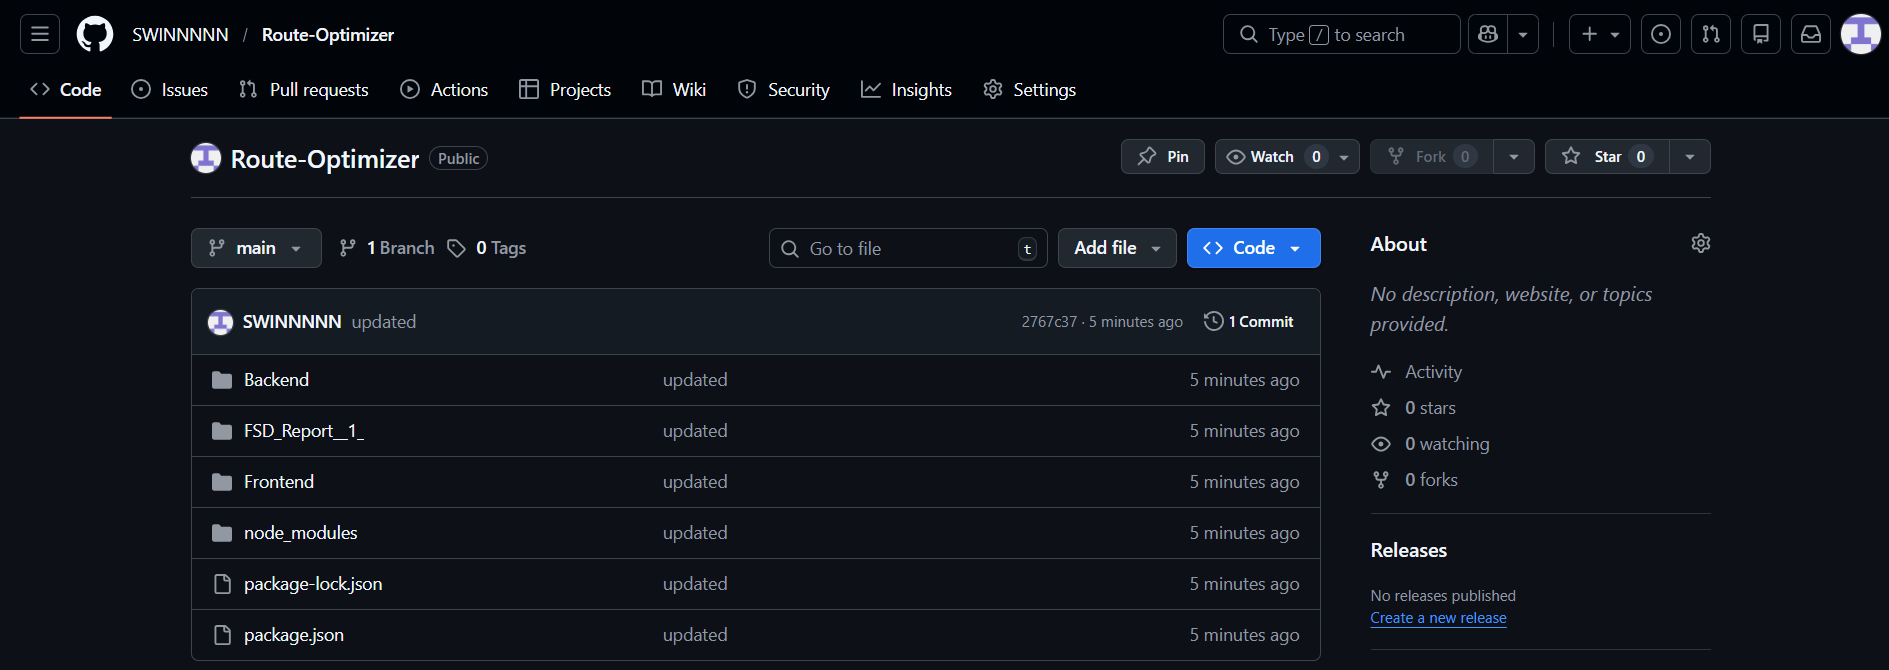
\includegraphics[width=1\textwidth]{git history/Repository overview.png}
    \caption{GitHub Repository Overview -- showing the main branch with project directories (Backend, Frontend, FSD\_Report) and configuration files hosted on the public repository.}
    \label{fig:git_repo_overview}
\end{figure}

\begin{figure}[H]
    \centering
    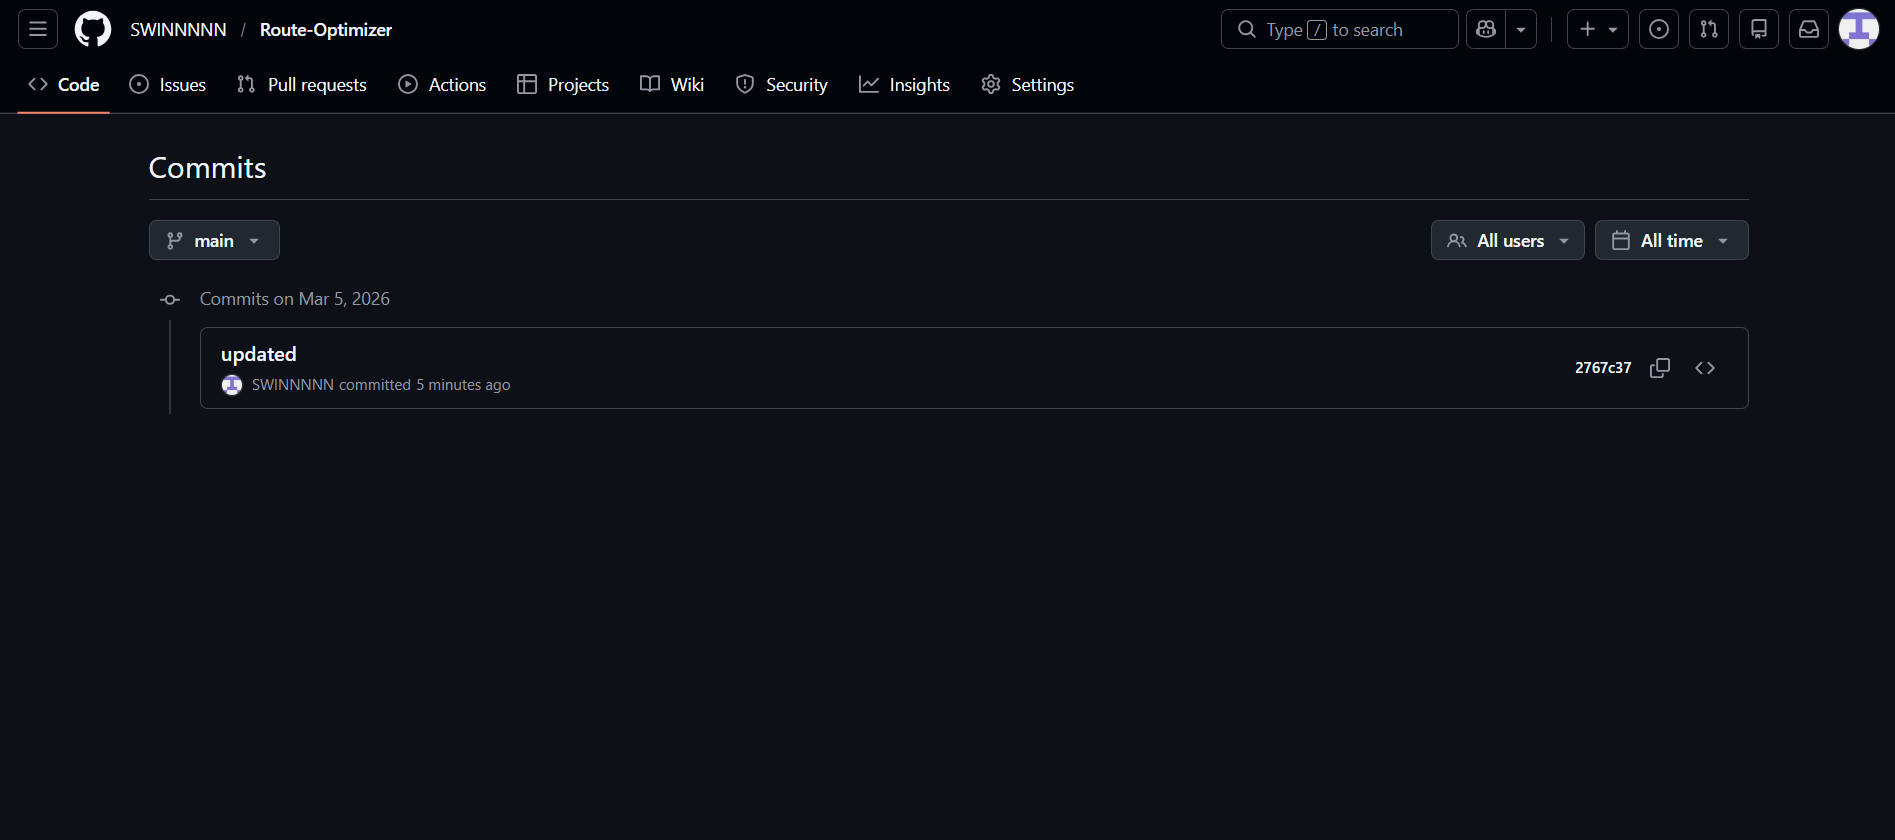
\includegraphics[width=1\textwidth]{git history/Commit detail.png}
    \caption{Git Commit History -- displaying the commit log on the main branch with the latest project update committed on Mar 5, 2026.}
    \label{fig:git_commit_detail}
\end{figure}